\subsection{Experimental method \& numerical model \label{sec:methods}} 
Methane pyrolysis experiments were conducted using the Stanford Flexible Applications Shock Tube (FAST) facility with a
3.35 m driver, 9.70 m driven section, and a 14.12 cm inner diameter. Fig.~\ref{fig:laserlayout} depicts a schematic of the diagnostic suite viewed from the end wall. More details about the FAST facility can be found in~\citep{rault2024multi}. The post-reflected shock pressure ($\mathrm{P_5}$) was measured using an endwall pressure transducer (Kistler 603B1). Time histories of key intermediates were quantified using laser absorption spectroscopy (LAS). C$_2$H$_4$ was measured at 10532~nm using an updated diagnostic technique originally developed by Ren et~al.~\citep{ren2012ir} and later refined by Pinkowski et~al.~\citep{pinkowski2019multi}. To reduce C$_2$H$_2$ interference with CH$_4$ absorption near 2998~nm~\citep{cassady2020thermal}, a NanoPlus distributed feedback laser was employed to detect C-H stretch vibrations of CH$_4$ at 3366~nm, with temperature-dependent absorption coefficients ($\sigma_v$) determined over 1500–2450~K and 1–5~atm. C$_2$H$_2$ was detected at 2998~nm using absorption cross-sections reported by Stranic et~al.~\citep{stranic2014laser}. To address CH$_4$ interference at 2998~nm, the absorption coefficient of CH$_4$ at this wavelength was also characterized for the range of experimental temperatures and pressures, allowing correction of the C$_2$H$_2$ measurements. % on the order of \textcolor{red}{XX}.

\begin{figure}[!t]
	\centering
	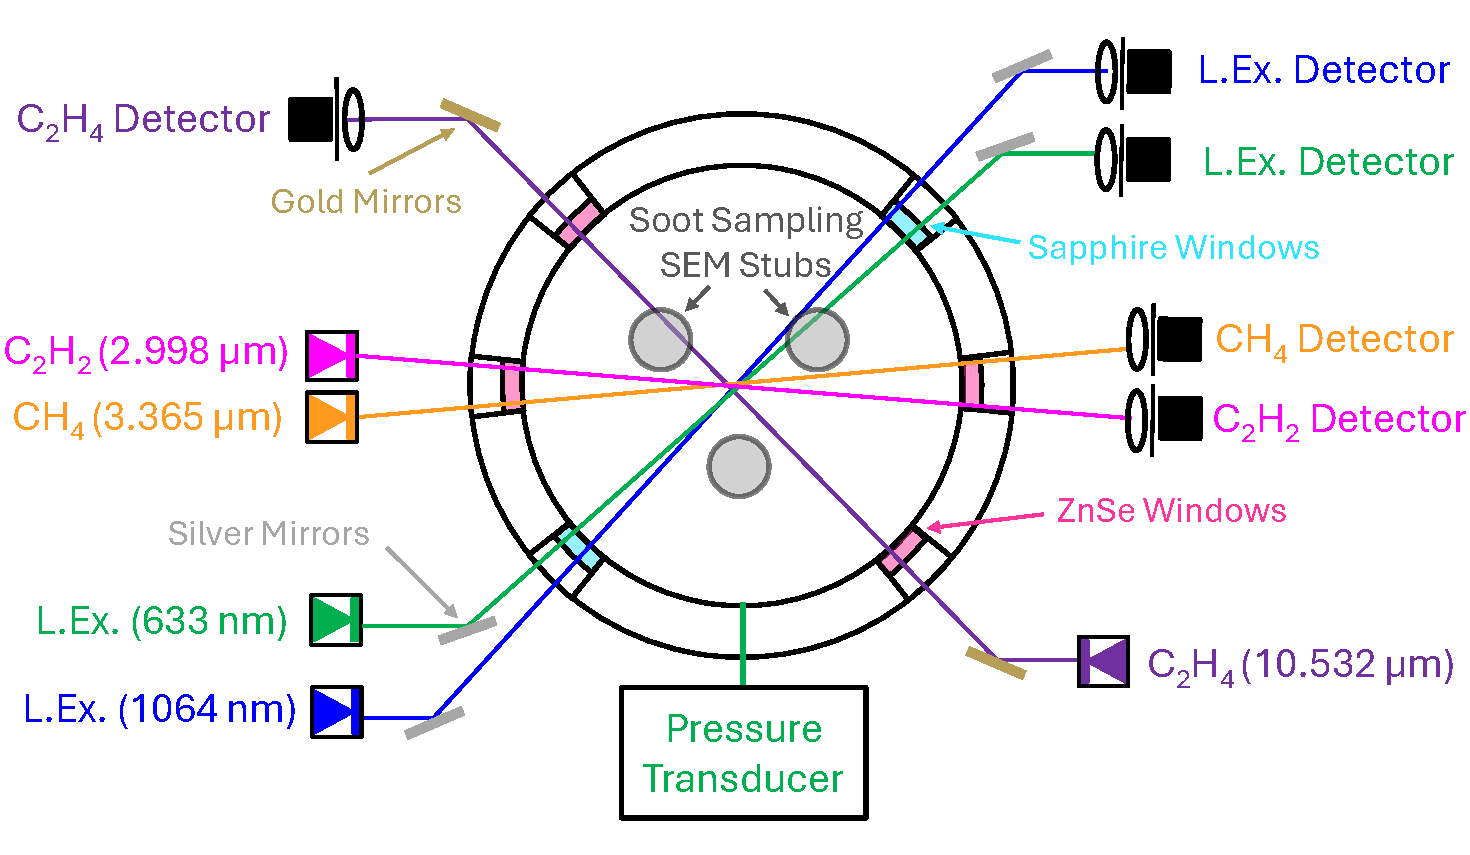
\includegraphics[width=0.7\textwidth]{Figures/Results/Paper2/laser_setup.pdf}
	\caption{Schematics of the laser diagnostics and shock-tube setup. Spatial and spectral filtering is employed to ensure high-quality absorbance measurements to infer species mole fractions and soot volume fraction. All lasers are aligned in a plane 1 cm from the endwall.}
	\label{fig:laserlayout} 
\end{figure}


Light extinction at $\lambda$=633~nm (Coherent Inc. 70 mW OBIS 633 nm LX laser) was employed to measure time-resolved volume fraction of soot particles with optical properties in the Rayleigh limit~\citep{eremin2012formation} as:

\begin{equation}
f_v =\ln\left(\frac{I_0}{I_t}\right)
\frac{\lambda}{6\pi\cdot L\cdot E(m)},
\end{equation}
\noindent where $L$=14.12~cm is the optical path length, and $E(m)$=[0.17, 0.26]~\citep{lee1981optical, dalzell1969optical} is the soot absorption function at 633~nm. 

The measured pressure trace was filtered to reduce noise and fluctuations, then applied to the pressure-reactor model in Omnisoot~\citep{adib2026omnisoot} to simulate methane pyrolysis in the shock tube. Four kinetic mechanisms were used to describe the gas-phase chemistry: ABF~\citep{appel2000kinetic}, KAUST~\citep{wang2013pah}, CRECK~\citep{pejpichestakul2019examination}, and FFCM2~\citep{ZDV2023}. All mechanisms except FFCM2 include PAH chemistry required for soot modeling and can therefore be coupled with a sectional population balance model. The \textit{BIN} species representing solid particles were removed from CRECK to avoid double-counting soot mass. Soot inception was modeled using a modified E-bridge formation based on the inception model proposed by Frenklach and Mebel~\citep{frenklach2020mechanism} with some modifications detailed in~\citep{adib2026omnisoot}. Surface growth was described by H-abstraction–C$_2$H$_2$/carbon-addition (HACA)~\citep{appel2000kinetic} and PAH adsorption. Soot precursors include naphthalene, phenanthrene, pyrene, acenaphthylene, acephenanthrylene, and cyclopentapyrene. An Arrhenius equation is used to account for the loss of hydrogen by the carbonization of soot particles as~\citep{basile2002coagulation}:

\begin{equation}
	\left(\frac{\mathrm{d}H_{tot}}{\mathrm{d}t}\right)_{\mathrm{carb}}=
	-A_{carb}\cdot \mathrm{exp}(\frac{-E_{carb}}{RT}),
	\label{eqn:kads_ebir}
\end{equation}

\noindent where $A_{carb}$=6$\times10^6$~[1/s] and $E_{carb}$=2$\times10^5$~[J/mol] are the exponential prefactor and activation energy for carbonization, respectively.